\chapter{Clúpiter}
\label{chap:conceptos_basicos}

\lettrine{P}{ara} comprender el objetivo del proyecto y su propuesta de valor, primero es necesario entender sus características, la justificación de las mismas, y el funcionamiento de sus componentes más primitivos.

\section{Nombre y marca corporativa}
Si bien este no es un elemento altamente importante en un proyecto de ingeniería como este, sí que es conveniente, y nunca está de más, otorgarle personalidad mediante la creación de un nombre e isotipo para el mismo.

El nombre del clúster es \textbf{Clúpiter} (ClúPIter): una mezcla entre las palabras ``Clúster'' y el ``PI'' de la \acrlong{rpi}, que de forma muy conveniente recuerda en su segunda parte a Júpiter. Este es a su vez planeta del sistema solar junto con el (enano) Plutón, nombre del clúster del \acrshort{gac}\footnote{\url{http://pluton.dec.udc.es}} (\acrlong{gac}). Es cuanto menos paradójico que el clúster en miniatura sea Júpiter, y el real sea Plutón\dots

En cuanto a la marca del clúster, éste no puede quedar sin un logo, que se muestra en la Figura \ref{fig:clupiter_logo}.\footnote{El uso del logo de Arch Linux sin autorización explícita está permitido en general para propósitos no comerciales. Clúpiter no tiene ningún tipo de vinculación con la marca Arch Linux (\url{https://wiki.archlinux.org/title/DeveloperWiki:TrademarkPolicy})}

\begin{figure}[h!]
  \centering
  \vspace*{0.5cm}
  \def\svgwidth{0.50\textwidth}
  \input{pdf_tex/clupiter_logo/clupiter_logo.pdf_tex}
  \caption{Logo de Clúpiter}
  \label{fig:clupiter_logo}
\end{figure}

\section{Clústeres}
Los clústeres, de los que para este proyecto se tratarán los de alto rendimiento, son conjuntos de ordenadores diseñados para ofrecer altas prestaciones de cálculo.

Estos clústeres pueden ser homogéneos o heterogéneos, siendo compuestos por computadores con la misma arquitectura y capacidades, o con arquitecturas o capacidades diferentes, respectivamente.

En el caso de Clúpiter, éste es un clúster muy homogéneo, ya que está compuesto por ocho mini-computadores exactamente iguales.

\section{Raspberry Pi 4 Model B}
\label{sec:raspberry_pi_4_model_b}
Cada aproximadamente dos años, la Raspberry Pi Foundation saca una nueva versión de su compacto y más exitoso producto: la \acrlong{rpi}, o por sus siglas \acrshort{rpi}. Estos pequeños computadores vienen en diversos formatos de forma, pero el que ha catapultado esta plataforma al éxito ha sido el formato que denominan \textit{Standard}\footnote{85.6 mm × 56.5 mm}.

Siendo cada versión mucho más potente que la anterior, y costando aproximadamente el mismo precio, está claro que la Raspberry Pi Foundation está haciendo un excelente trabajo aportando valor a este segmento del bajo consumo y coste.

La \acrlong{rpi} 4B (4 Model B) es la versión más nueva de formato \textit{Standard}, y por ello ha sido la elección para constituir la base del clúster.

\subsection{¿Hardware libre?}
Si bien multitud de componentes software de la \acrlong{rpi} son libres, como por ejemplo el kernel de Linux, las coreutils (habitualmente de la GNU) o la librería OpenMPI, de la que hablo más adelante, la \acrlong{rpi} no se puede considerar completamente libre.

Sí es cierto que la fundación publica esquemáticos con un buen nivel de detalle acerca del interconexionado entre las piezas, así como completas guías de referencia, pero la placa en sí no es hardware libre. Primero porque sus componentes no han sido ni publicados ni diseñados con tecnologías libres, y segundo porque la \acrlong{rpi} Foundation se reserva el derecho de fabricación de esta placa. 

\section{MPI}
Para aprovechar todo el potencial hardware de los supercomputadores y, en general, de los computadores paralelos, existen paradigmas de programación específicos. \acrshort{mpi} (\acrlong{mpi})\footnote{\url{https://www.mpi-forum.org}} es un estándar para la programación de los sistemas paralelos de memoria distribuida como Clúpiter.

Como no podría ser de otra forma, siguiendo el espíritu open source, y también por conveniencia, ya que es la librería MPI que ofrece Arch Linux  en
sus repositorios oficiales, y contra la que se compilan por defecto sus ejecutables, en este proyecto se emplea una implementación libre de MPI: \textbf{OpenMPI}, licenciada bajo la BSD. 

\section{Estructura hardware}
La estructura física y lógica de Clúpiter es completamente abierta, y se puede encontrar descrita en las siguientes Figuras (\ref{fig:raspi_diagram_eth}, \ref{fig:raspi_electric_diagram}).

\begin{figure}[h!]
  \centering
  \vspace{0.10cm}
  \resizebox{0.8\linewidth}{!}{
  \def\svgwidth{0.9\textwidth}
  \input{pdf_tex/raspi_diagram_eth/raspi_diagram.pdf_tex}
  }
  \caption{Esquema físico de red de Clúpiter}
  \label{fig:raspi_diagram_eth}
\end{figure}

\begin{figure}[h!]
  \centering
  \vspace{0.15cm}
  \def\svgwidth{0.9\textwidth}
  \input{pdf_tex/electric_diagram/electric_diagram.pdf_tex}
  \caption{Diagrama eléctrico de Clúpiter}
  \label{fig:raspi_electric_diagram}
  \vspace{0.15cm}
\end{figure}

Clúpiter montado se muestra a continuación, en las Figuras \ref{fig:fotos_estructura_top} y \ref{fig:fotos_estructura_bottom}.

\begin{figure}[H]
    \centering
    \begin{subfigure}[c]{0.45\textwidth}
        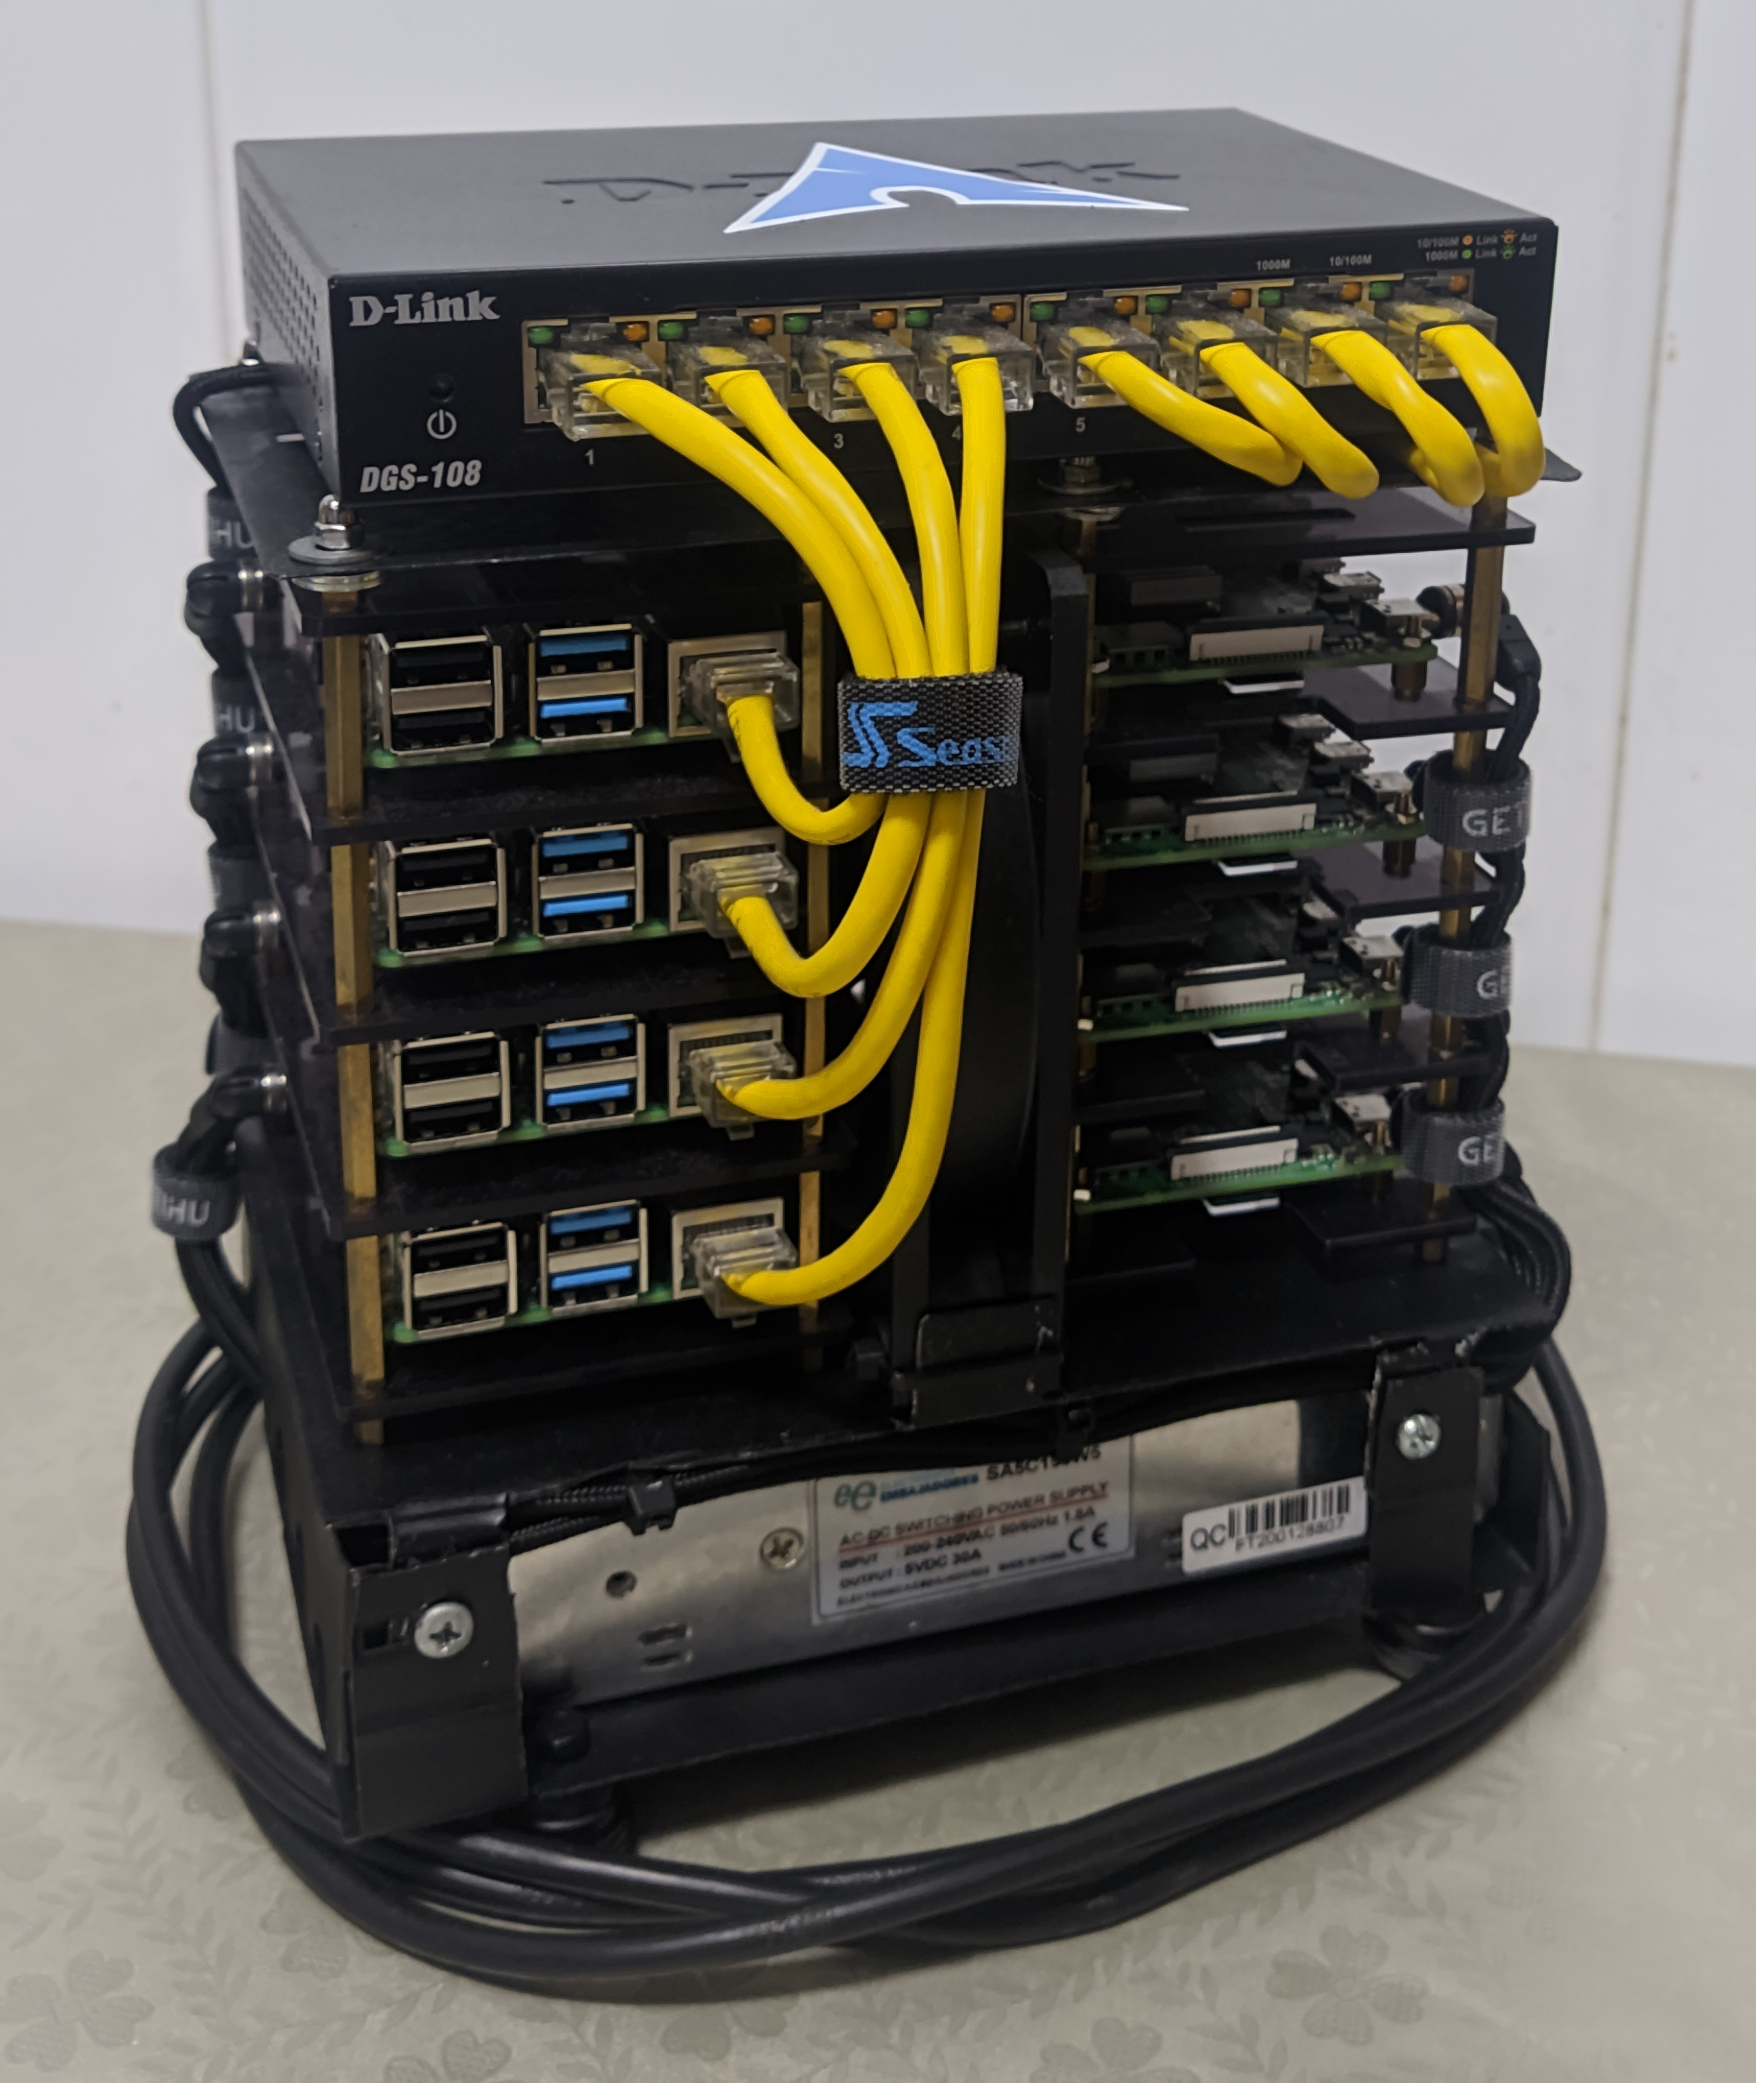
\includegraphics[width=\textwidth]{img/top.jpg}
        \caption{Clúpiter en picado}
        \label{fig:fotos_estructura_top}
    \end{subfigure}
    \begin{subfigure}[c]{0.45\textwidth}
        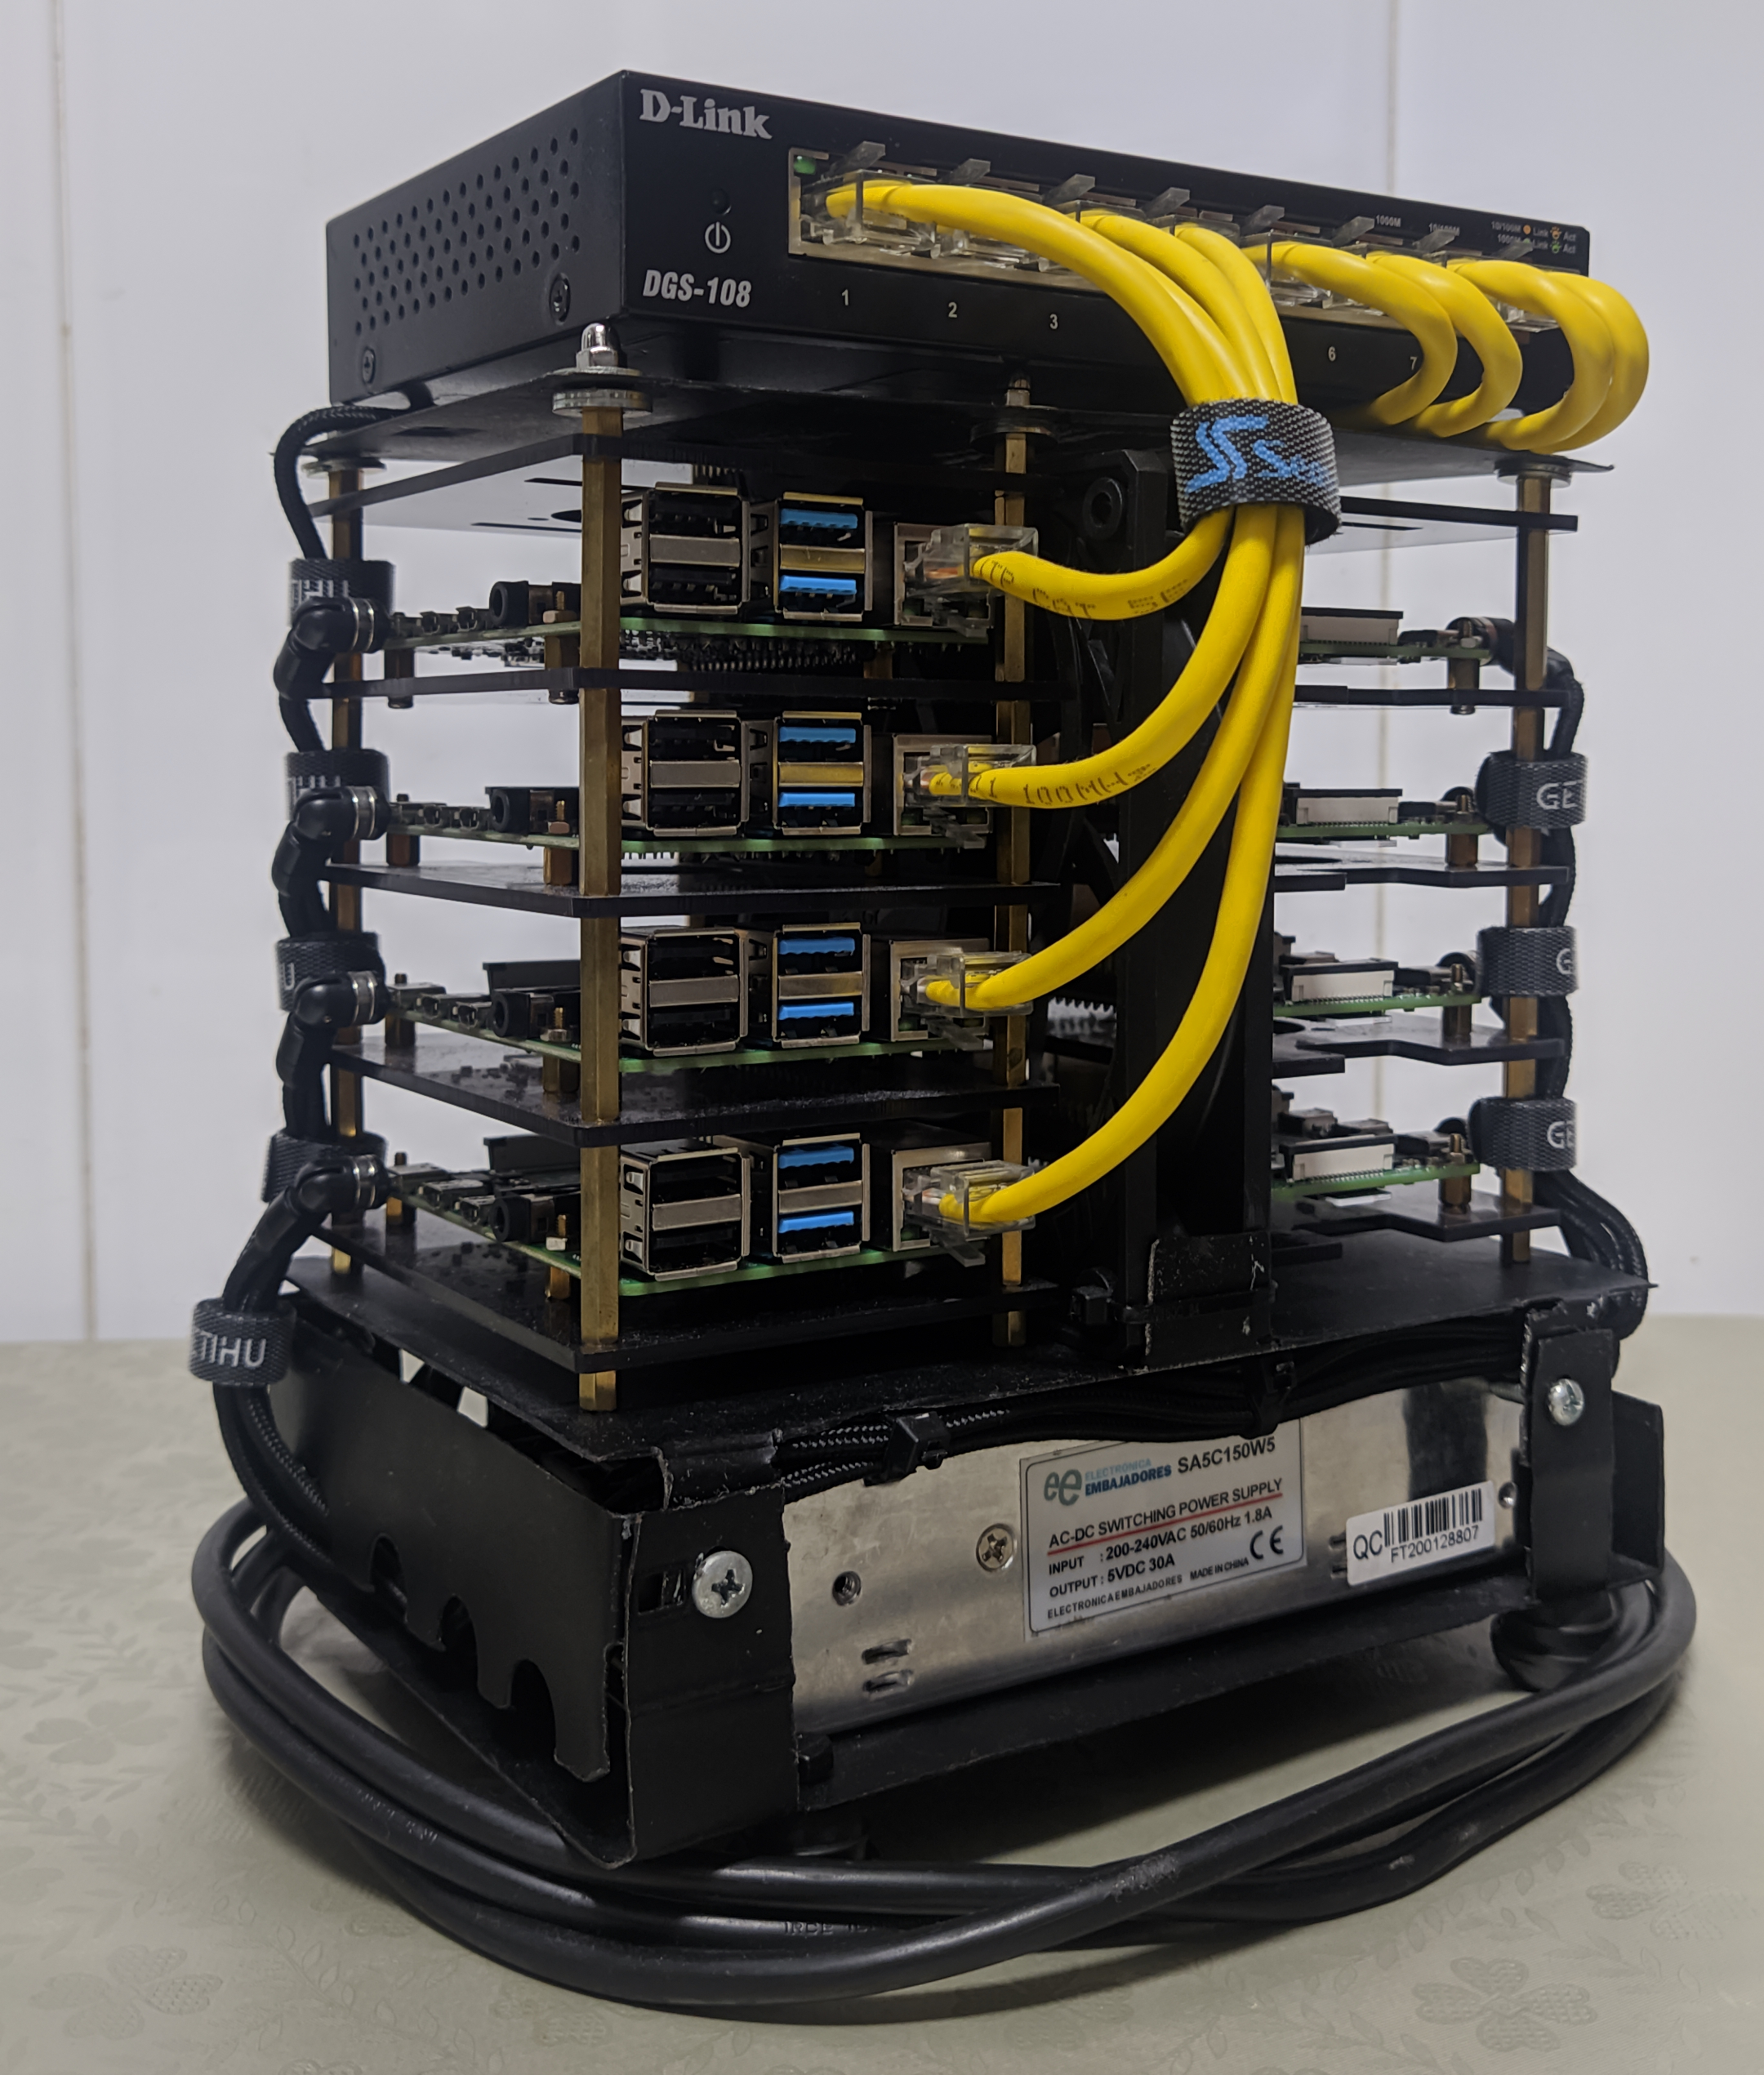
\includegraphics[width=\textwidth]{img/bottom.jpg}
        \caption{Clúpiter en contrapicado}
        \label{fig:fotos_estructura_bottom}
    \end{subfigure}
    \label{fig:fotos_estructura}
    \caption{Clúpiter completamente ensamblado}
\end{figure}
